% Entrega 3: informe final (mismo formato de las Entregas 1 y 2).
% Compilar con: xelatex informe_final.tex (dos veces)
\documentclass[11pt,a4paper]{article}
\usepackage[top=2.3cm,bottom=2.2cm,left=2.2cm,right=2.2cm,headsep=0.7cm]{geometry}
\usepackage{fontspec}
\setmainfont{Liberation Serif}
\usepackage{babel}
\babelprovide[import,main]{spanish}
\usepackage{microtype}
\usepackage{tabularx,array,booktabs}
\usepackage{enumitem}
\usepackage{titlesec}
\usepackage{caption}
\usepackage{graphicx}
\usepackage{fancyhdr}
\usepackage{tikz}
\usetikzlibrary{positioning,arrows.meta}
\usepackage[hidelinks]{hyperref}
\urlstyle{rm}

\AtBeginDocument{\renewcommand{\tablename}{Tabla}\renewcommand{\figurename}{Figura}}
\linespread{1.04}
\setlength{\parskip}{3pt}
\setlength{\parindent}{1.2em}
\titleformat{\section}{\large\bfseries}{\thesection.}{0.5em}{}
\titlespacing*{\section}{0pt}{11pt}{4pt}
\setlist{itemsep=1pt,topsep=3pt,parsep=0pt,leftmargin=1.5em}
\captionsetup{font=small,labelfont=bf,labelsep=period,skip=4pt,justification=justified,singlelinecheck=false}
\setlength{\textfloatsep}{10pt plus 2pt minus 2pt}
\setlength{\floatsep}{8pt plus 2pt minus 2pt}
\setlength{\intextsep}{9pt plus 2pt minus 2pt}
\newcommand{\code}[1]{\textit{#1}}
\newcolumntype{Y}{>{\raggedright\arraybackslash}X}
\setlength{\emergencystretch}{2em}
\renewcommand{\topfraction}{0.85}\renewcommand{\bottomfraction}{0.6}\renewcommand{\textfraction}{0.12}\renewcommand{\floatpagefraction}{0.8}

\pagestyle{fancy}
\fancyhf{}
\fancyhead[L]{\small\textit{Técnicas Avanzadas de Modelado · Entrega 3}}
\fancyhead[R]{\small\textit{Reconocimiento de señas aisladas LSC-54}}
\fancyfoot[C]{\small\thepage}
\renewcommand{\headrulewidth}{0.4pt}
\fancypagestyle{plain}{\fancyhf{}\fancyfoot[C]{\small\thepage}\renewcommand{\headrulewidth}{0pt}}

\begin{document}

\thispagestyle{plain}
\begin{center}
{\Large\bfseries Reconocimiento de señas aisladas de la Lengua de Señas Colombiana:\\[3pt] una red recurrente sobre landmarks frente a una línea base clásica}\\[8pt]
{\normalsize Andrés Díaz, Lorena Valero, Jorge Anaya y Sabrina Miranda}\\[3pt]
{\small Maestría en Analítica Aplicada e Inteligencia Artificial, Universidad de La Sabana}\\
{\small Técnicas Avanzadas de Modelado, 2026-II \,·\, Entrega 3: informe final \,·\, Octubre de 2026}\\[2pt]
{\small\url{https://github.com/andresdila/lsc54-reconocimiento-senas}}
\end{center}
\vspace{2pt}
\noindent\rule{\textwidth}{0.4pt}

\begin{quote}\small
\noindent\textbf{Resumen.} Se clasifican 43 señas aisladas de la campaña S2 del conjunto LSC-54 a partir de landmarks de MediaPipe, siempre sobre personas que no participaron en el entrenamiento. Se compara una regresión logística sobre estadísticas por video, que actúa como línea base, con una GRU bidireccional con atención temporal de 552.023 parámetros. En validación cruzada agrupada por señante (14 señantes, 7 folds), el macro-F1 pasa de 0,548 $\pm$ 0,166 a 0,811 $\pm$ 0,079, con mejora en los 7 folds; en el test bloqueado (4 señantes, evaluado una sola vez) pasa de 0,685 a 0,881. El costo de entrenamiento sube de 0,9 s a 227 s, con una latencia de 6,8 ms por video en CPU. El desempeño varía mucho entre personas (de 0,69 a 0,92 en test), los números son la familia de señas más confundida, el modelo es sobreconfiado y cuatro señantes de prueba no bastan para garantizar una generalización amplia.
\end{quote}
\vspace{-4pt}
\noindent\rule{\textwidth}{0.4pt}

%--------------------------------------------------------------------------------------
\section{Problema, contexto y alcance}

La Lengua de Señas Colombiana (LSC) es la lengua de la comunidad sorda del país, y el acceso a su aprendizaje formal sigue siendo limitado. El conjunto LSC-54 se construyó para respaldar una herramienta de enseñanza de vocabulario básico (Mora-Zarate et al., 2025), y este proyecto adopta ese propósito: un estudiante practica frente a una cámara y recibe retroalimentación sobre si la seña ejecutada corresponde a la solicitada. De ahí se desprende la unidad de generalización del experimento; como el sistema siempre se enfrentará a una persona nueva, toda evaluación se hace sobre señantes ausentes del entrenamiento.

El problema es una clasificación multiclase de señas aisladas: dado un video corto, se asigna una de 43 etiquetas, 33 expresiones de cortesía y los números del uno al diez. Se ubica entre las series de tiempo y la visión por computador, porque MediaPipe (Lugaresi et al., 2019) convierte cada video en una serie multivariada de coordenadas de manos y torso, y es esa serie, no los píxeles, la que recibe el modelo. Quedan fuera del alcance la lengua de señas continua, la traducción, la campaña de colores (S1), el reconocimiento en tiempo real y cualquier despliegue con usuarios sordos sin su validación previa.

\textbf{Pregunta experimental.} Bajo una partición independiente del señante, ¿un modelo secuencial sobre landmarks mejora el macro-F1 frente a una línea base clásica sobre estadísticas de los landmarks, y a qué costo computacional? La hipótesis es que la dinámica temporal del movimiento aporta información que los resúmenes estadísticos pierden. Con solo 14 señantes de desarrollo no era obvio que se cumpliera, así que la comparación se diseñó para poder rechazarla con la misma claridad con que podía aceptarse.

%--------------------------------------------------------------------------------------
\section{Datos: procedencia, licencia y auditoría de calidad}

LSC-54 fue publicado por Mora-Zarate, Garzón-Castro y Castellanos-Rivillas (2025) en \emph{Data in Brief}, con DOI del conjunto 10.57760/sciencedb.25639 y licencia CC BY-NC 4.0, que permite el uso académico y no comercial con atribución. Por esta razón los videos no se redistribuyen en el repositorio; \code{download\_data.py} los obtiene de la fuente oficial y verifica su MD5. Los autores reportan 54 señas, 22 participantes y entre tres y cinco repeticiones por seña. La versión aumentada $\times$45 (51,4 GB) no se usa, porque multiplicar los videos antes de particionar es una fuente clásica de fuga de información (Scikit-learn Developers, s.~f.).

El inventario real contiene 2.850 videos sin duplicados. Se trabaja con la campaña S2, de cortesía y números: 1.740 videos únicos, 43 clases y 18 señantes. Se excluye S1 porque su numeración de carpetas es independiente de la de S2 y no permite garantizar que una misma persona no quede a ambos lados de la partición. La extracción procesó los 1.740 videos (113.658 cuadros) sin dejar ninguno vacío. La pose se detecta en el 99,5\,\% de los cuadros, pero la mano más activa solo en el 60\,\%, probablemente porque las manos en reposo no se detectan. El 32\,\% de los videos queda bajo el 50\,\% de detección de manos; se conservan, ya que excluirlos eliminaría un tercio de los datos, y la tasa de detección se usa como eje del análisis de errores. La detección varía mucho entre personas, de 0,46 (S2-19) a 0,97 (S2-32), y es mayor en los señantes de test (0,73) que en los de desarrollo (0,57), lo que anticipa un desempeño de test algo optimista.

%--------------------------------------------------------------------------------------
\section{Partición y protocolo de evaluación}

La partición v1 se versionó antes de extraer landmarks o entrenar cualquier modelo, y se hace sobre señantes y nunca sobre videos: las repeticiones de una persona se parecen entre sí, de modo que una división por video mediría la memorización de la identidad y no la generalización a personas nuevas (Scikit-learn Developers, s.~f.; Zinkevich, s.~f.). La Tabla~\ref{tab:particion} resume el esquema.

\begin{table}[htbp]
\centering
\caption{Partición v1 por señante (semilla 2026).}\label{tab:particion}
\small
\renewcommand{\arraystretch}{1.18}
\begin{tabularx}{\textwidth}{@{}>{\raggedright\arraybackslash}p{3.2cm}cc Y@{}}
\toprule
\textbf{Partición} & \textbf{Señantes} & \textbf{Videos} & \textbf{Composición}\\
\midrule
Desarrollo (folds 1 a 7) & 14 & 1.359 & 7 folds de 192 a 206 videos; cada fold valida con 1 señante que graba las 43 clases (\emph{full}) y 1 que graba 21 (\emph{partial})\\
Test bloqueado & 4 & 381 & S2-01 y S2-03 (\emph{full}); S2-29 y S2-31 (\emph{partial})\\
\bottomrule
\end{tabularx}
\end{table}

La estratificación por tipo de cobertura garantiza que las 43 clases estén en el test y en cada fold, pero implica que 22 clases se validan con un único señante en cada fold, es decir, con unos tres videos. Por eso el macro-F1 por fold es ruidoso y se reporta también sobre las predicciones fuera de muestra de los siete folds agrupadas. Las medidas contra la fuga de información son pruebas automáticas que verifican que ningún señante aparezca en dos particiones, incluida una que planta una fuga y comprueba que se detecta; un \code{make\_split.py -{}-check-only} que se niega a sobrescribir la partición; el ajuste de la imputación y la estandarización dentro de cada fold; la selección de hiperparámetros solo con desarrollo; y un test que se evalúa una única vez, con scripts que se niegan a repetirlo.

Las reglas de decisión se fijaron en el plan, antes de ver resultados secuenciales. El modelo candidato se considera mejor si su macro-F1 en validación cruzada supera al de la línea base en al menos 0,05 y mejora en al menos 5 de los 7 folds; la diferencia se acompaña de un intervalo de confianza por remuestreo de señantes y no de un valor $p$ aislado, y el test bloqueado solo confirma la decisión final. La métrica principal es el macro-F1, que da el mismo peso a las 43 clases; como secundarias se reportan la exactitud, el top-3, el F1 por clase y por señante, y el costo (parámetros, tiempo de ajuste y latencia).

%--------------------------------------------------------------------------------------
\section{Método}

\textbf{Preprocesamiento común.} MediaPipe Holistic 0.10.21 entrega, por cuadro, siete puntos de pose del tren superior y 21 puntos por mano, es decir, 98 valores $(x, y)$. No se usan landmarks faciales, por parsimonia y para reducir la identificabilidad de las personas. Como MediaPipe normaliza $x$ por el ancho e $y$ por el alto, y los videos tienen dos resoluciones (640$\times$360 y 640$\times$480), las coordenadas se pasan a píxeles antes de normalizar; de lo contrario, el modelo podría aprender qué cámara se usó y no qué seña se hizo. Luego se centran en el punto medio de los hombros y se escalan por la distancia entre ellos. Las manos no detectadas quedan como ausentes, y esa información se conserva.

\textbf{Línea base.} Cada video se resume en 493 variables (media, desviación, mínimo, máximo y velocidad media absoluta de cada coordenada, tasa de detección de cada mano y número de cuadros), que alimentan un \emph{pipeline} de scikit-learn con imputación por mediana, estandarización y regresión logística multinomial (C = 1; 21.242 parámetros). Se acompaña de dos referencias triviales, la clase mayoritaria y el muestreo por frecuencia, que fijan el piso: el macro-F1 de la clase mayoritaria es 0,001.

\textbf{Modelo avanzado.} La secuencia se remuestrea a 32 cuadros, se interpolan vacíos de hasta 5 cuadros, se agregan tres canales de máscara de presencia (pose, mano izquierda y mano derecha) y el logaritmo del número de cuadros entra a la cabeza. Una proyección lineal 101$\rightarrow$128 con LayerNorm alimenta dos capas de GRU bidireccional (Cho et al., 2014) de 128 unidades; una atención temporal produce un vector por video, y una capa densa con dropout de 0,3 entrega las 43 probabilidades (Figura~\ref{fig:flujo}). Se entrena con entropía cruzada y AdamW (Loshchilov y Hutter, 2019), con calentamiento lineal de 5 épocas, descenso coseno, recorte del gradiente en 1,0 y 80 épocas fijas. Los aumentos (recorte temporal, escala, rotación de $\pm$10° y ruido gaussiano, sin reflejo horizontal para no alterar la lateralidad) se aplican solo en entrenamiento. Se reporta la métrica de la última época, porque elegir la mejor época con el fold de validación inflaría la estimación: la mejor época promedia 0,831, frente a 0,811 de la última.

\begin{figure}[htbp]
\centering
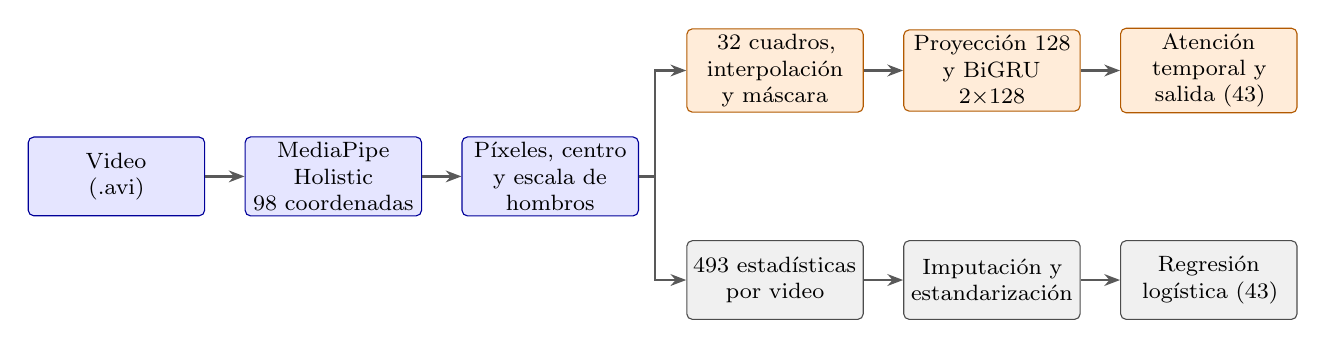
\begin{tikzpicture}[
  node distance=4mm and 5mm,
  box/.style={draw, rounded corners=2pt, align=center, font=\footnotesize, minimum height=10mm, text width=21mm, inner sep=2pt},
  shared/.style={box, fill=blue!10, draw=blue!60!black},
  seq/.style={box, fill=orange!15, draw=orange!70!black},
  base/.style={box, fill=gray!12, draw=gray!60!black},
  arr/.style={-{Stealth[length=2mm]}, thick, gray!70!black}]
\node[shared] (v) {Video\\(.avi)};
\node[shared, right=of v] (mp) {MediaPipe Holistic\\98 coordenadas};
\node[shared, right=of mp] (nm) {Píxeles, centro y escala de hombros};
\node[seq, above right=3mm and 6mm of nm] (rs) {32 cuadros, interpolación y máscara};
\node[seq, right=of rs] (gru) {Proyección 128 y BiGRU 2$\times$128};
\node[seq, right=of gru] (att) {Atención temporal y salida (43)};
\node[base, below right=3mm and 6mm of nm] (st) {493 estadísticas por video};
\node[base, right=of st] (lr) {Imputación y estandarización};
\node[base, right=of lr] (rl) {Regresión logística (43)};
\draw[arr] (v) -- (mp); \draw[arr] (mp) -- (nm);
\draw[arr] (nm.east) -- ++(2mm,0) |- (rs.west); \draw[arr] (nm.east) -- ++(2mm,0) |- (st.west);
\draw[arr] (rs) -- (gru); \draw[arr] (gru) -- (att);
\draw[arr] (st) -- (lr); \draw[arr] (lr) -- (rl);
\end{tikzpicture}
\caption{Flujo completo del sistema. Azul: preprocesamiento compartido; naranja: modelo secuencial; gris: línea base.}\label{fig:flujo}
\end{figure}

La Tabla~\ref{tab:config} reúne la configuración completa de la BiGRU base (\code{configs/model.yaml}), que es la que se evalúa en el test.

\begin{table}[htbp]
\centering
\caption{Configuración de la BiGRU base.}\label{tab:config}
\small
\renewcommand{\arraystretch}{1.18}
\begin{tabularx}{\textwidth}{@{}>{\raggedright\arraybackslash}p{2.3cm}Y>{\raggedright\arraybackslash}p{2.3cm}Y@{}}
\toprule
\textbf{Grupo} & \textbf{Parámetros} & \textbf{Grupo} & \textbf{Parámetros}\\
\midrule
Datos & 32 cuadros; vacíos de hasta 5 cuadros interpolados; plausibilidad de 6 anchos de hombro; máscara y duración activas & Aumentos & Recorte temporal 0,10; escala 0,10; rotación 10°; ruido 0,01; solo en entrenamiento\\
Modelo & Proyección 128; GRU bidireccional de 2 capas de 128; dropout 0,3 (cabeza) y 0,1 (recurrente) & Entrenamiento & AdamW, tasa $10^{-3}$, weight decay 0,01; lote 32; 80 épocas; calentamiento 5 y coseno; recorte 1,0\\
Semilla & 2026 más el número de fold & Evaluación & Última época, sin parada temprana ni selección de época\\
\bottomrule
\end{tabularx}
\end{table}

%--------------------------------------------------------------------------------------
\section{Resultados en validación cruzada por señante}

La Tabla~\ref{tab:cv} compara los modelos con los mismos 7 folds. La BiGRU supera a la regresión logística en los 7 folds (Figura~\ref{fig:validacion}a), con una diferencia media por fold de +0,263; sobre las predicciones agrupadas la diferencia es de +0,244, con intervalo del 95\,\% por remuestreo de señantes (2.000 réplicas) de +0,16 a +0,37. Ambas cifras quedan muy por encima del umbral de 0,05 fijado de antemano, de modo que se cumple la regla de decisión. La conclusión se mantiene si se aplica a la línea base el mismo filtro de plausibilidad que usa la BiGRU: la diferencia es de +0,251, con intervalo de +0,16 a +0,35. El peor señante pasa de 0,108 (S2-19, con una de las detecciones de manos más bajas, 0,46) a 0,527 (S2-21).

\begin{table}[htbp]
\centering
\caption{Validación cruzada agrupada por señante. Macro-F1 como media $\pm$ desviación estándar entre los 7 folds; la columna agrupada se calcula sobre las predicciones fuera de muestra de los 7 folds juntas.}\label{tab:cv}
\small
\renewcommand{\arraystretch}{1.18}
\begin{tabularx}{\textwidth}{@{}Ycccccc@{}}
\toprule
\textbf{Modelo} & \textbf{Macro-F1} & \textbf{Agrupado} & \textbf{Exactitud} & \textbf{Top-3} & \textbf{Peor señante} & \textbf{Parámetros}\\
\midrule
Clase mayoritaria & 0,001 & 0,003 & 0,032 & 0,079 & --- & ---\\
Regresión logística$^{\ast}$ & 0,548 $\pm$ 0,166 & 0,572 & 0,569 & 0,782 & 0,108 & 21.242\\
\textbf{BiGRU base} & \textbf{0,811 $\pm$ 0,079} & \textbf{0,816} & \textbf{0,811} & \textbf{0,923} & \textbf{0,527} & 552.023\\
\bottomrule
\end{tabularx}
\par\smallskip
\begin{minipage}{\textwidth}\footnotesize
$^{\ast}$ Las predicciones fuera de muestra de la línea base se recalcularon en la máquina de los experimentos para compararlas video a video; su macro-F1 es 0,548 $\pm$ 0,166, frente a 0,549 $\pm$ 0,167 en la Entrega 1, una diferencia numérica atribuible al entorno de cómputo.
\end{minipage}
\end{table}

\begin{figure}[htbp]
\centering
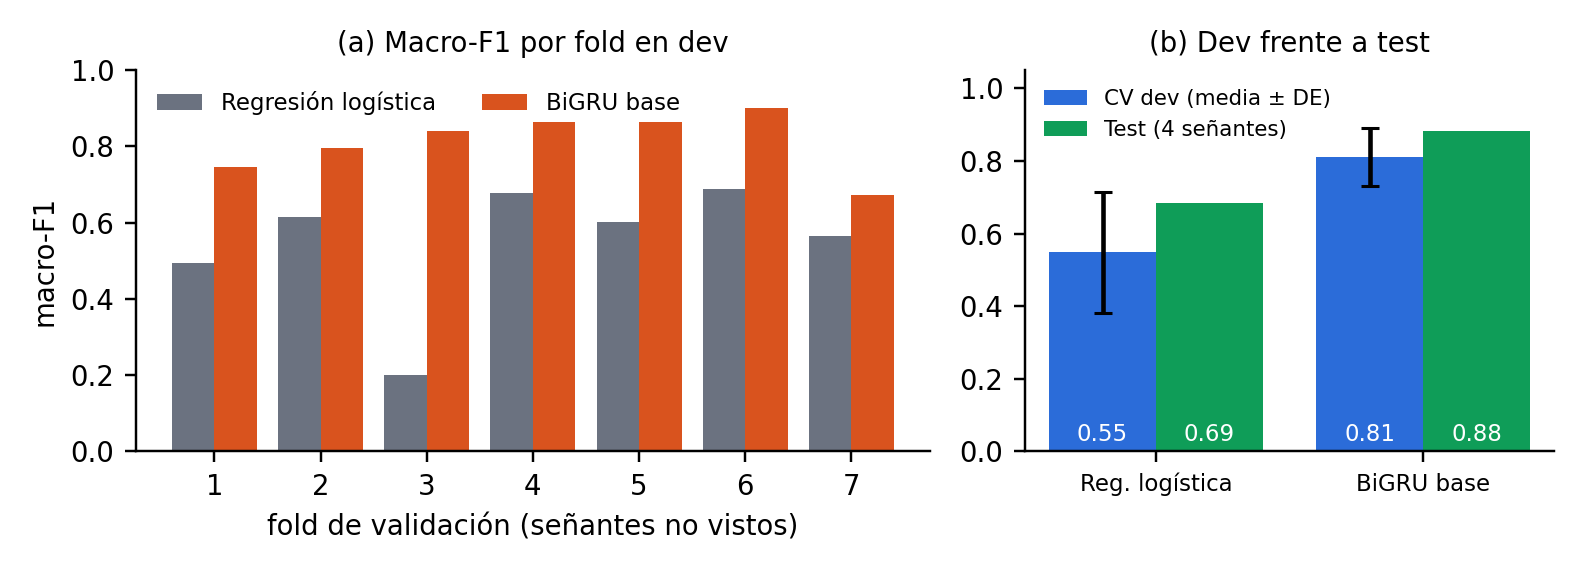
\includegraphics[width=0.82\textwidth]{figures/fig2_validacion.png}
\caption{(a) Macro-F1 por fold de validación. (b) Macro-F1 medio en validación cruzada (barras de error: desviación estándar entre folds) y en el test bloqueado.}\label{fig:validacion}
\end{figure}

\textbf{Experimentos controlados.} Se ejecutaron 14 variantes que cambian un solo factor respecto a la base (Godbole et al., 2023), con la misma partición y semilla (Figura~\ref{fig:experimentos} y Tabla~\ref{tab:experimentos}). Para que la tabla y el texto usen la misma medida, la diferencia frente a la base se calcula siempre sobre las predicciones agrupadas, con su intervalo por remuestreo de señantes. Se destacan tres resultados. Primero, el optimizador es el factor con mayor efecto en esta configuración: Adam con L2 acoplado (0,599) y SGD con Nesterov (0,635) quedan más cerca de la línea base que de AdamW (0,811). Sin embargo, ambos se probaron con la tasa de aprendizaje y el weight decay de la base, sin reajustarlos, y su macro-F1 de entrenamiento se queda en 0,79 a 0,80 en la época 80, cuando AdamW ya está en 1,0; se trata de un subajuste, de modo que el resultado describe su comportamiento con esa configuración y no una superioridad general de AdamW. Segundo, los aumentos aportan unos 0,04 (0,771 sin ellos) y la GRU rinde más que la LSTM (0,754) con la misma configuración. Tercero, las señales de calidad de los datos ayudan poco, pero de forma consistente: quitar la máscara de presencia o la duración reduce el macro-F1 en 0,016 y 0,020, con intervalos que no incluyen el cero, lo que descarta que la duración sea un atajo dominante.

\begin{figure}[htbp]
\centering
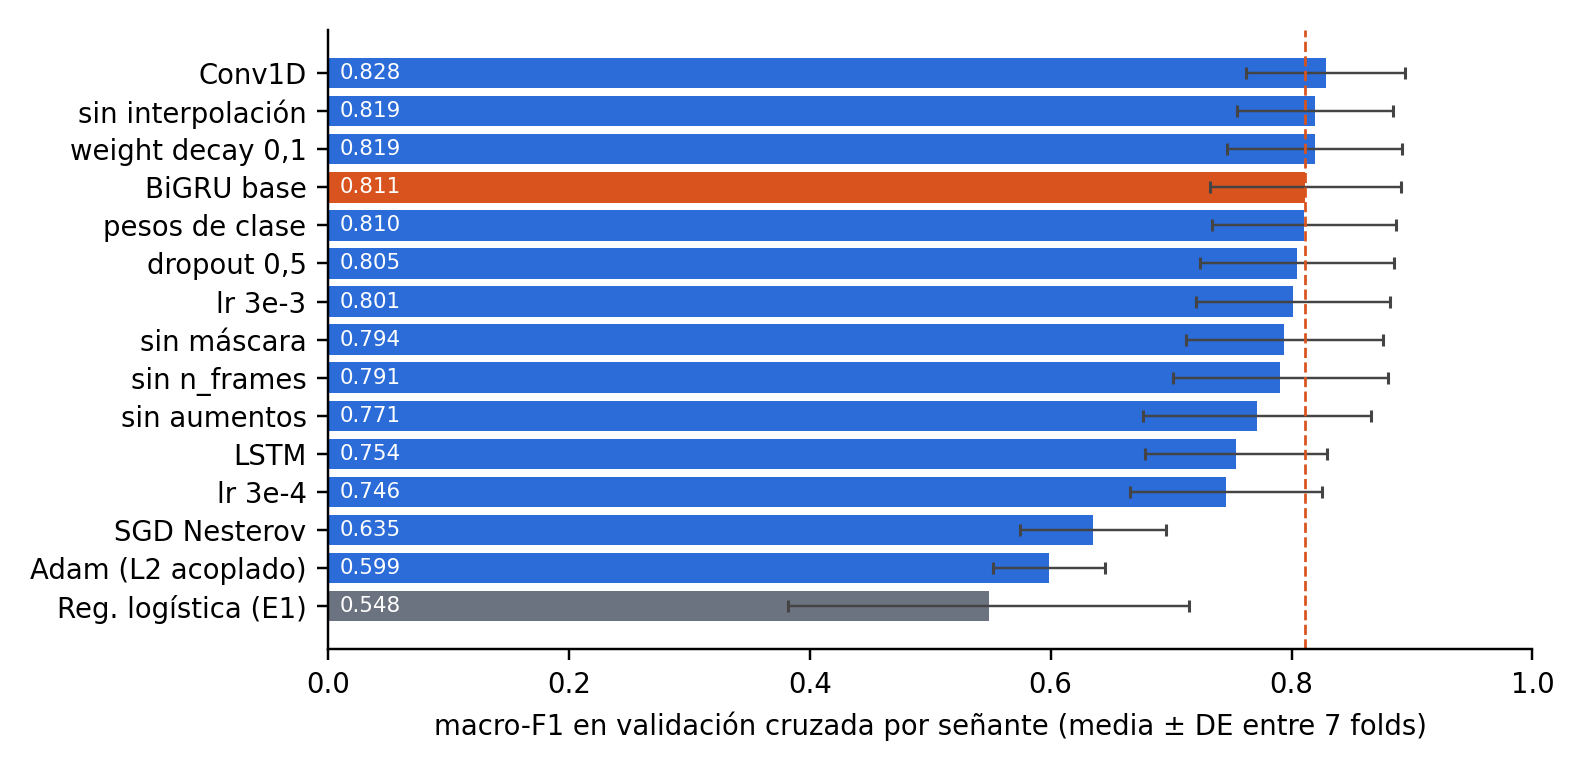
\includegraphics[width=0.74\textwidth]{figures/fig3_experimentos.png}
\caption{Macro-F1 en validación cruzada de la línea base y de las 14 variantes (media $\pm$ desviación estándar entre folds). La línea punteada marca la BiGRU base.}\label{fig:experimentos}
\end{figure}

\begin{table}[htbp]
\centering
\caption{Experimentos de un factor a la vez (validación cruzada, 7 folds). Macro-F1: media de folds; $\Delta$: diferencia de macro-F1 agrupado frente a la base, con IC del 95\,\% por remuestreo de señantes (1.000 réplicas; 2.000 para la línea base).}\label{tab:experimentos}
\small
\renewcommand{\arraystretch}{1.12}
\begin{tabularx}{\textwidth}{@{}l Y c c c c@{}}
\toprule
\textbf{Experimento} & \textbf{Factor que cambia} & \textbf{Macro-F1} & \textbf{$\Delta$ [IC 95\,\%]} & \textbf{Peor señante} & \textbf{s/fold}\\
\midrule
conv1d & Codificador Conv1D & 0,828 & +0,019 [$-$0,011; +0,044] & 0,641 & 154\\
wd0.1 & Weight decay 0,1 & 0,819 & +0,006 [$-$0,005; +0,020] & 0,542 & 184\\
sin\_interpolacion & Sin interpolación de vacíos & 0,819 & +0,005 [$-$0,008; +0,019] & 0,570 & 180\\
\textbf{base} & \textbf{Configuración base} & \textbf{0,811} & --- & \textbf{0,527} & $\approx$183$^{\dagger}$\\
pesos\_clase & Pesos de clase & 0,810 & $-$0,002 [$-$0,013; +0,010] & 0,540 & 196\\
dropout0.5 & Dropout 0,5 & 0,805 & $-$0,006 [$-$0,023; +0,010] & 0,549 & 183\\
lr3e-3 & Tasa $3\times10^{-3}$ & 0,801 & $-$0,014 [$-$0,029; +0,007] & 0,531 & 185\\
sin\_mascara & Sin máscara de presencia & 0,794 & $-$0,016 [$-$0,033; $-$0,001] & 0,536 & 185\\
sin\_ncuadros & Sin duración del video & 0,791 & $-$0,020 [$-$0,038; $-$0,003] & 0,536 & 248\\
sin\_aumentos & Sin aumentos & 0,771 & $-$0,040 [$-$0,077; $-$0,014] & 0,525 & 190\\
lstm & Codificador LSTM & 0,754 & $-$0,057 [$-$0,085; $-$0,035] & 0,516 & 173\\
lr3e-4 & Tasa $3\times10^{-4}$ & 0,746 & $-$0,063 [$-$0,085; $-$0,047] & 0,497 & 183\\
opt\_sgd & SGD con Nesterov & 0,635 & $-$0,167 [$-$0,202; $-$0,126] & 0,494 & 180\\
opt\_adam & Adam con L2 acoplado & 0,599 & $-$0,196 [$-$0,241; $-$0,150] & 0,493 & 183\\
logreg & Línea base (Entrega 1) & 0,548 & $-$0,244 [$-$0,37; $-$0,16] & 0,108 & 1,8\\
\bottomrule
\end{tabularx}
\par\smallskip
\begin{minipage}{\textwidth}\footnotesize
$^{\dagger}$ El tiempo de la corrida base (427 s) estaba inflado por el modo de ahorro de batería; se reporta el de las variantes con la misma arquitectura.
\end{minipage}
\end{table}

Las tres variantes que superan a la base lo hacen por menos de 0,02, con intervalos que incluyen el cero. Elegir la mejor de 14 variantes evaluadas en los mismos folds inflaría la estimación por sesgo de selección; por ello se conservó la BiGRU base, que era la candidata registrada antes de ver resultados, y estas variantes se reportan como oportunidades de mejora y no como ganancias. El empate de la Conv1D tiene, además, una implicación de fondo: un codificador convolucional, que también lee el orden de los cuadros pero sin recurrencia, alcanza el mismo desempeño con 154 s por fold y 0,7 ms por video. Por tanto, la ganancia frente a la línea base proviene de modelar la secuencia y no de la recurrencia en sí, y la Conv1D sería la candidata natural para un uso en tiempo real.

Las curvas de aprendizaje (Figura~\ref{fig:curvas}) muestran el comportamiento esperado con pocos señantes. En promedio, el macro-F1 de entrenamiento alcanza 0,99 en la época 41, mientras que el de validación se estabiliza en 0,81 y no cae. La pérdida de validación, en cambio, toca su mínimo en la época 27 (0,81; entre la época 15 y la 47 según el fold) y termina en 0,93, un 15\,\% por encima. La red memoriza a los señantes de entrenamiento y se vuelve cada vez más segura de sus predicciones, también de las equivocadas; la entropía cruzada lo castiga aunque los aciertos no disminuyan, lo que anticipa la sobreconfianza que se cuantifica en la Sección~\ref{sec:errores}. Los aumentos y la regularización mitigan este sobreajuste, pero no lo eliminan, y la dispersión entre folds es grande (de 0,67 a 0,90).

\begin{figure}[htbp]
\centering
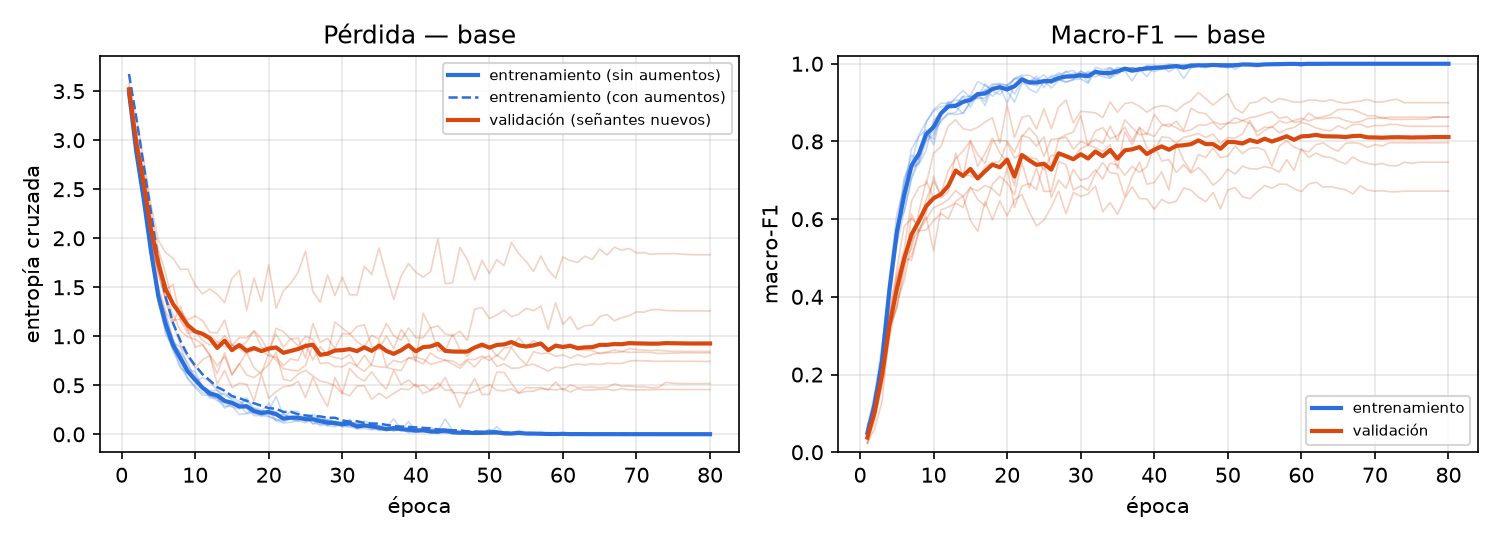
\includegraphics[width=0.84\textwidth]{figures/fig4_curvas.png}
\caption{Curvas de entrenamiento y validación de la BiGRU base. Líneas gruesas: promedio de los 7 folds; líneas finas: cada fold.}\label{fig:curvas}
\end{figure}

%--------------------------------------------------------------------------------------
\section{Decisiones de modelado y validez de la comparación}

\textbf{Justificación de las decisiones.} Una red recurrente encaja con el problema porque una seña es una secuencia con orden y duración variables; la bidireccionalidad permite usar el contexto en ambos sentidos al clasificar un video completo, y la atención temporal evita que el vector final dependa solo del último cuadro. Remuestrear a 32 cuadros, cuando la mediana de los videos es 53, uniformiza la entrada con poca pérdida de información y mantiene bajo el costo. Se prefirió la GRU sobre la LSTM porque cumple la misma función con un 23\,\% menos de parámetros (552.023 frente a 716.887), y la ablación respalda la elección (0,811 frente a 0,754). Se eligió el macro-F1 para que las 22 clases con menor cobertura de señantes no queden eclipsadas por las 21 más frecuentes, y un número fijo de épocas para no usar el fold de validación como criterio de parada.

\textbf{Qué hace válida la comparación.} Ambos modelos usan los mismos 1.359 videos de desarrollo, los mismos 7 folds, la misma semilla y el mismo preprocesamiento, con todo ajuste dependiente de los datos dentro de cada fold. La candidata, la regla de decisión y sus umbrales se registraron antes de ver resultados secuenciales, y la decisión sobre el test se registró antes de evaluarlo.

\textbf{Ajuste de la línea base.} La línea base se fijó con C = 1, mientras que el modelo avanzado recibió 14 exploraciones, aunque ninguna se usó para seleccionarlo. Para medir cuánto de la brecha podría deberse a esa asimetría, se evaluaron con los mismos folds y las mismas 493 variables la regresión logística con C entre 0,01 y 10, un bosque aleatorio de 500 árboles y una SVM con kernel RBF (\code{scripts/tune\_baseline.py}; Tabla~\ref{tab:sensibilidad}). La mejor opción, la regresión logística con C = 10, alcanza 0,554 $\pm$ 0,163, apenas por encima de C = 1. Escoger la mejor de siete opciones con los mismos folds favorece a la línea base; aun así, la brecha con la BiGRU sigue siendo de 0,26, de modo que no se explica por falta de ajuste.

\begin{table}[htbp]
\centering
\caption{Sensibilidad de la línea base: macro-F1 en validación cruzada (media $\pm$ desviación estándar entre folds) con las mismas 493 variables.}\label{tab:sensibilidad}
\small
\renewcommand{\arraystretch}{1.18}
\begin{tabularx}{\textwidth}{@{}YYYYYYY@{}}
\toprule
\multicolumn{4}{c}{\textbf{Regresión logística}} & \textbf{Bosque} & \multicolumn{2}{c}{\textbf{SVM RBF}}\\
\cmidrule(lr){1-4}\cmidrule(l){6-7}
C = 0,01 & C = 0,1 & C = 1 & C = 10 & \textbf{aleatorio} & C = 1 & C = 10\\
\midrule
0,319 $\pm$ 0,085 & 0,492 $\pm$ 0,145 & 0,549 $\pm$ 0,167 & \textbf{0,554 $\pm$ 0,163} & 0,511 $\pm$ 0,112 & 0,247 $\pm$ 0,062 & 0,475 $\pm$ 0,145\\
\bottomrule
\end{tabularx}
\end{table}

\textbf{Qué debilita la comparación.} (i) No se probaron métodos de \emph{gradient boosting}, que podrían reducir parte de la brecha, aunque los resultados de la Tabla~\ref{tab:sensibilidad} lo hacen poco probable; (ii) la línea base resume los datos con estadísticas que descartan el orden temporal, de modo que la comparación mide a la vez el valor del orden y el de una representación más rica; (iii) los 14 experimentos comparten folds, por lo que sus errores están correlacionados; (iv) cada configuración se entrenó con una sola semilla por fold, así que la dispersión refleja a las personas y no la variación del entrenamiento; y (v) los tiempos provienen de una sola máquina con CPU. Estas salvedades no invierten el resultado, pero impiden afirmar que la BiGRU sea la mejor opción posible; sí muestran que supera a esta línea base, en estas condiciones, por un margen que excede el ruido.

%--------------------------------------------------------------------------------------
\section{Evaluación final en el test bloqueado}

El 22 de octubre de 2026 se registró la decisión (BiGRU base, sin cambios, commit \code{dbbe611}) antes de tocar el test. Ambos modelos se entrenaron una vez con los 14 señantes de desarrollo y se evaluaron una única vez sobre los 4 señantes de test (381 videos), con el commit \code{9431af2} y el árbol de trabajo limpio (Tabla~\ref{tab:test}).

\begin{table}[htbp]
\centering
\caption{Test bloqueado (4 señantes, 381 videos) y costo computacional (CPU, 8 hilos).}\label{tab:test}
\small
\renewcommand{\arraystretch}{1.18}
\begin{tabularx}{\textwidth}{@{}Yccc@{}}
\toprule
\textbf{Métrica} & \textbf{Regresión logística} & \textbf{BiGRU base} & \textbf{Diferencia}\\
\midrule
Macro-F1 & 0,685 & \textbf{0,881} & +0,196\\
Exactitud & 0,669 & \textbf{0,869} & +0,200\\
Top-3 & 0,829 & \textbf{0,955} & +0,126\\
Tiempo de ajuste (desarrollo completo) & 0,9 s & 227 s & $\approx$250$\times$\\
Latencia por video (en lote / individual) & 0,01 ms / n.\,d. & 0,39 ms / 6,8 ms & ---\\
Parámetros & 21.242 & 552.023 & $\approx$26$\times$\\
\bottomrule
\end{tabularx}
\end{table}

El test respalda la dirección y el tamaño del efecto observados en validación cruzada: la BiGRU gana en los cuatro señantes, y el intervalo de la diferencia por remuestreo de señantes va de +0,09 a +0,35. Hay, sin embargo, dos razones para no tomar 0,881 como la expectativa para cualquier persona nueva. La primera es que los señantes de test tienen mejor detección de manos que los de desarrollo (0,73 frente a 0,57), algo que el plan ya identificaba como fuente de optimismo. La segunda es la dispersión entre personas: S2-03 obtiene 0,924, S2-01 0,901, S2-29 0,819 y S2-31 0,687 (Figura~\ref{fig:senantes}a). Con cuatro señantes, el intervalo es amplio, y la cifra de validación cruzada (0,811 $\pm$ 0,079) es la mejor referencia de cuánto puede variar el desempeño. En cuanto al costo, la BiGRU es unas 250 veces más lenta de entrenar, pero 6,8 ms por video en CPU son compatibles con una herramienta de práctica interactiva, en la que la extracción con MediaPipe, de unos 2,5 s por video, domina la latencia.

\textbf{Uso del test durante el entrenamiento final.} El script del entrenamiento final reutiliza la misma función que en los folds y, por ello, calcula las métricas del test al cierre de cada época. Esas curvas no se guardaron ni se consultaron; el número de épocas (80) estaba fijado desde la validación cruzada, y el modelo evaluado es el de la última época. El test, por tanto, no intervino en ninguna decisión. Aun así, en una versión posterior conviene que el entrenamiento final no reciba el test hasta terminar, de modo que la garantía quede en el código y no solo en el procedimiento.

%--------------------------------------------------------------------------------------
\section{Análisis de errores y calibración}\label{sec:errores}

De los 381 videos de test, 50 se clasificaron mal (13\,\%): 12 de S2-01, 9 de S2-03, 10 de S2-29 y 19 de S2-31. Diez de las 43 clases alcanzan F1 = 1,0. Los errores se concentran en los números: la confusión más frecuente es seis $\rightarrow$ uno (6 videos; el F1 de «seis», 0,375, es el más bajo), seguida de cuatro $\rightarrow$ tres, nueve $\rightarrow$ ocho y ocho $\rightarrow$ siete, es decir, números contiguos (Tabla~\ref{tab:confusiones}). Entre las señas de cortesía destacan bien $\rightarrow$ por favor (3) y lo siento $\rightarrow$ por favor (2). El patrón se repite en validación cruzada: el F1 medio de los números es 0,71, frente a 0,85 de las expresiones de cortesía, y las clases más difíciles son «sí» (0,50), «necesitar» (0,52), «no» (0,55), «uno» (0,56) y «seis» (0,56). Una hipótesis plausible, que este trabajo no probó, es que los números difieren en la configuración de los dedos, un detalle fino que 21 puntos por mano en dos dimensiones capturan mal cuando la detección falla o es imprecisa; la coordenada de profundidad o los ángulos entre dedos serían la prueba natural. Con 6 a 13 videos por clase en test, los F1 por clase son indicativos y no concluyentes.

\begin{table}[htbp]
\centering
\caption{Confusiones más frecuentes en el test (50 errores en 381 videos; las otras 26 combinaciones ocurren una vez cada una).}\label{tab:confusiones}
\small
\renewcommand{\arraystretch}{1.12}
\begin{tabular}{@{}llc@{\hspace{2.2em}}llc@{}}
\toprule
\textbf{Real} & \textbf{Predicha} & \textbf{Videos} & \textbf{Real} & \textbf{Predicha} & \textbf{Videos}\\
\midrule
seis & uno & 6 & bien & diez & 2\\
bien & por favor & 3 & baño & mal & 2\\
cuatro & tres & 3 & hola & tres & 2\\
nueve & ocho & 2 & lo siento & por favor & 2\\
ocho & siete & 2 & & & \\
\bottomrule
\end{tabular}
\end{table}

La variación entre personas es la fuente de incertidumbre dominante (Tabla~\ref{tab:senantes}). El peor señante de test, S2-31, es también el único de los 18 con una detección de pose claramente menor (0,89, frente a una mediana cercana a 1,0) y concentra 19 de los 50 errores con solo 61 videos; falla el 31\,\% de sus videos, frente al 7 a 16\,\% de los demás (Figura~\ref{fig:senantes}b). Esto es coherente con la hipótesis de que la calidad de detección condiciona el desempeño, pero se trata de un solo señante y no permite afirmar causalidad. Tampoco es una relación simple: S2-03, con una detección media de manos de 0,51, obtiene 0,92. La comparación con la línea base apunta en la misma dirección desde otro ángulo. En S2-19, una de las personas con menor detección de manos (0,46), la regresión logística obtiene 0,11 y la BiGRU 0,87, probablemente porque los resúmenes estadísticos se contaminan con los vacíos de detección, mientras que la secuencia con máscara e interpolación los maneja mejor; la ablación sin máscara ($-$0,016) respalda de forma modesta esa lectura.

\begin{table}[htbp]
\centering
\caption{Macro-F1 por señante (desarrollo: predicciones fuera de muestra de la validación cruzada; test: modelos finales) y detección media de manos.}\label{tab:senantes}
\small
\renewcommand{\arraystretch}{1.08}
\begin{tabular}{@{}lccc@{\hspace{2.6em}}lccc@{}}
\toprule
\textbf{Señante} & \textbf{Detección} & \textbf{Reg. log.} & \textbf{BiGRU} & \textbf{Señante} & \textbf{Detección} & \textbf{Reg. log.} & \textbf{BiGRU}\\
\midrule
S2-17 & 0,46 & 0,66 & 0,85 & S2-28 & 0,54 & 0,50 & 0,74\\
S2-19 & 0,46 & 0,11 & 0,87 & S2-30 & 0,84 & 0,67 & 0,75\\
S2-21 & 0,48 & 0,46 & 0,53 & S2-32 & 0,97 & 0,54 & 0,73\\
S2-22 & 0,55 & 0,63 & 0,78 & S2-33 & 0,54 & 0,48 & 0,87\\
S2-23 & 0,65 & 0,46 & 0,72 & S2-34 & 0,64 & 0,67 & 0,84\\
S2-24 & 0,55 & 0,72 & 0,93 & S2-01 (test) & 0,89 & 0,55 & 0,90\\
S2-25 & 0,55 & 0,58 & 0,74 & S2-03 (test) & 0,51 & 0,86 & 0,92\\
S2-26 & 0,48 & 0,69 & 0,97 & S2-29 (test) & 0,79 & 0,58 & 0,82\\
S2-27 & 0,55 & 0,59 & 0,93 & S2-31 (test) & 0,79 & 0,37 & 0,69\\
\bottomrule
\end{tabular}
\end{table}

\begin{figure}[htbp]
\centering
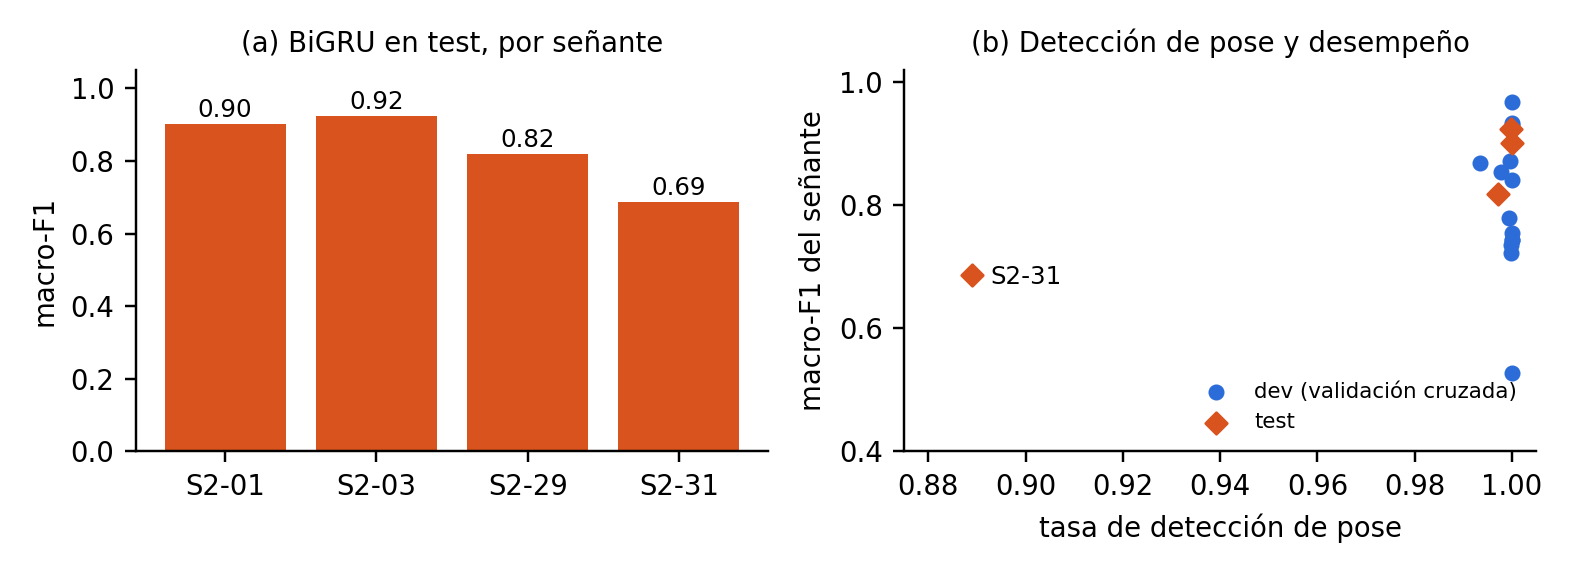
\includegraphics[width=0.82\textwidth]{figures/fig5_senantes.png}
\caption{(a) Macro-F1 de la BiGRU en test por señante. (b) Macro-F1 de cada señante (desarrollo en validación cruzada; test con el modelo final) frente a su tasa de detección de pose.}\label{fig:senantes}
\end{figure}

\textbf{Calibración.} Para una herramienta que muestre probabilidades o que se abstenga ante una baja confianza, no basta con acertar; las probabilidades deben corresponder a la frecuencia real de acierto. Sobre las predicciones fuera de muestra de la validación cruzada, la confianza media de la BiGRU es 0,925, mientras que su exactitud es 0,812, y el error de calibración esperado (ECE, 15 intervalos) es 0,114. Incluso cuando se equivoca, su confianza media es 0,77, en línea con el patrón de las curvas: el modelo es sobreconfiado. En consecuencia, un umbral de abstención basado en las probabilidades sin corregir dejaría pasar muchos errores. Antes de cualquier uso, conviene recalibrar con escalado de temperatura sobre las predicciones fuera de muestra, un ajuste de un solo parámetro que no cambia la clase predicha. Como apoyo práctico, cuando la BiGRU se equivoca, la seña correcta está entre sus tres primeras opciones en el 59\,\% de los casos (\code{scripts/report\_numbers.py}).

%--------------------------------------------------------------------------------------
\section{Limitaciones, riesgos y recomendaciones de uso}

La Tabla~\ref{tab:riesgos} contrasta los riesgos identificados en el plan, que sigue el marco de gestión de riesgos de inteligencia artificial del NIST (National Institute of Standards and Technology, 2023), con la evidencia obtenida. Además, hay tres limitaciones generales. El alcance léxico es de 43 señas aisladas de una sola campaña, y reconocer vocabulario aislado no equivale a comprender la lengua, que incluye gramática, expresión facial y uso del espacio; los landmarks faciales se excluyeron a propósito. La incertidumbre estadística es alta, porque algunos folds validan clases con un único señante, los intervalos por remuestreo de señantes son amplios y el test tiene solo cuatro personas. Por último, la licencia CC BY-NC 4.0 impide el uso comercial.

\begin{table}[htbp]
\centering
\caption{Riesgos de sesgo, privacidad y uso indebido: evidencia, mitigación y estado.}\label{tab:riesgos}
\small
\renewcommand{\arraystretch}{1.15}
\begin{tabularx}{\textwidth}{@{}>{\raggedright\arraybackslash}p{2.6cm}YY@{}}
\toprule
\textbf{Riesgo} & \textbf{Evidencia} & \textbf{Mitigación y estado}\\
\midrule
Representatividad & 18 señantes sin metadatos demográficos (no se sabe si son sordos, oyentes o intérpretes); solo 4 en test & Desempeño por señante reportado (0,69 a 0,92 en test); conclusiones limitadas a este grupo\\
Fuga de identidad & 38 identidades por carpeta (20 en S1 y 18 en S2) frente a 22 participantes & S1 excluido; partición por señante; pruebas automáticas con fuga plantada. Controlado\\
Detección desigual & Detección de manos de 0,46 a 0,97 entre señantes; S2-31 (pose 0,89) tiene el peor F1 de test & Medida y reportada; avisar al usuario cuando sea baja. Pendiente probar con más personas\\
Atajos no lingüísticos & La duración, la detección y la resolución podrían delatar al señante o a la cámara & Conversión a píxeles antes de normalizar; ablaciones sin duración ($-$0,020) y sin máscara ($-$0,016): no son atajos dominantes\\
Desbalance y cobertura & 26 a 57 videos por clase; 22 clases con solo 9 señantes & Macro-F1 como métrica principal; pesos de clase sin efecto ($-$0,002); F1 por clase reportado\\
Sobreconfianza & ECE de 0,114; confianza media de 0,77 en los errores & Recalibrar con escalado de temperatura antes de definir un umbral de abstención. Pendiente\\
Privacidad & Rostros pixelados por los autores; licencia CC BY-NC & No se redistribuyen videos; solo inventario y métricas; sin landmarks faciales\\
Uso indebido & Las señas aisladas no equivalen a la lengua; un error afecta a quien aprende & No usar como traductor; validar con la comunidad sorda y con docentes; mostrar el top-3 y abstenerse con baja confianza\\
\bottomrule
\end{tabularx}
\end{table}

\textbf{Recomendaciones de uso.} El modelo es apto como apoyo a la práctica de vocabulario básico, siempre que muestre las tres señas más probables (top-3 de 0,955 en test) y no una sola respuesta. No debe presentarse como traductor, ni sustituir a intérpretes, ni usarse para evaluar o calificar a personas. Antes de cualquier uso real se requiere validarlo con la comunidad sorda y con docentes de LSC, contar con datos de más personas y condiciones, recalibrar sus probabilidades y definir un umbral de confianza por debajo del cual el sistema se abstenga. La Tabla~\ref{tab:ficha} resume la ficha del modelo y de los datos; la versión completa está en \code{MODEL\_CARD.md} (Mitchell et al., 2019; Gebru et al., 2021).

\begin{table}[htbp]
\centering
\caption{Ficha resumida del modelo y de los datos.}\label{tab:ficha}
\small
\renewcommand{\arraystretch}{1.15}
\begin{tabularx}{\textwidth}{@{}>{\raggedright\arraybackslash}p{2.8cm}Y@{}}
\toprule
\textbf{Campo} & \textbf{Contenido}\\
\midrule
Modelo & BiGRU de 2 capas (128 unidades) con atención temporal; 552.023 parámetros; entrada de 32 cuadros con 98 coordenadas y máscara; salida de 43 clases\\
Uso previsto & Retroalimentación en la práctica de vocabulario básico de LSC (cortesía y números), con una persona frente a una cámara\\
Usos no previstos & Traducción, interpretación, evaluación de personas, reconocimiento de lengua continua, uso comercial y vigilancia\\
Datos & LSC-54, campaña S2: 1.740 videos, 18 señantes, 43 clases; CC BY-NC 4.0; sin rostros (landmarks de manos y torso)\\
Desempeño & Macro-F1 de 0,811 $\pm$ 0,079 en validación cruzada por señante; 0,881 en test (4 señantes, optimista por mejor detección)\\
Calibración y costo & ECE de 0,114 (sobreconfianza); 227 s de entrenamiento y 6,8 ms por video en CPU\\
Riesgos principales & Variación entre personas (0,69 a 0,92 en test), confusión entre números contiguos y dependencia de la calidad de detección\\
\bottomrule
\end{tabularx}
\end{table}

%--------------------------------------------------------------------------------------
\section{Reproducibilidad}

El repositorio reproduce todo el flujo con Python 3.11 o 3.12 y \code{mediapipe==0.10.21}, versión que no funciona con Python 3.13 o superior y que se necesita para extraer los landmarks. Cada JSON de resultados registra la semilla (2026), la versión de la partición, el hash del commit, si el árbol estaba limpio y las versiones de Python (3.11.17), PyTorch (2.14.1+cpu), scikit-learn (1.9.1) y NumPy (1.26.4). Los comandos, en orden, son los siguientes; la extracción tarda unos 45 minutos y el entrenamiento de la base, unos 35 minutos en CPU:

\noindent\begin{minipage}{\textwidth}\begin{quote}\small
\texttt{python scripts/download\_data.py}\\
\texttt{python scripts/make\_split.py --check-only}\\
\texttt{python scripts/extract\_landmarks.py --workers 2}\\
\texttt{python scripts/train\_baseline.py --model logreg}\\
\texttt{python scripts/train\_sequence.py --name base}\\
\texttt{python scripts/run\_experiments.py}\\
\texttt{python scripts/compare\_models.py --candidate base}\\
\texttt{python scripts/tune\_baseline.py}\\
\texttt{python scripts/report\_numbers.py}\\
\texttt{pytest -q}
\end{quote}\end{minipage}


El test bloqueado no forma parte de esta secuencia: los scripts se niegan a repetir \code{-{}-final-test}, y los resultados de la evaluación única ya están versionados en \code{reports/e1\_plan/} y \code{reports/e3\_final/}. Las 22 pruebas automáticas incluyen los controles contra la fuga de información. El mismo experimento base, reentrenado en otra máquina (Linux), dio un macro-F1 de 0,808 $\pm$ 0,079 frente a 0,811 $\pm$ 0,079, con diferencias por fold de a lo sumo 0,03. Cinco de los 14 experimentos registran \code{git\_dirty: true} porque Git en Windows reportaba el bit de permisos de ejecución como un cambio; el contenido de \code{src/}, \code{scripts/}, \code{configs/} y \code{splits/} es idéntico al del commit. Los mensajes de los commits se reescribieron antes de publicar las ramas, por lo que los resúmenes antiguos citan \code{bbbc4a4}, equivalente a \code{dbbe611} por tener el mismo árbol de archivos. Queda pendiente fijar las versiones exactas en un \code{requirements.lock}.

%--------------------------------------------------------------------------------------
\section{Conclusiones y oportunidades de mejora}

Con señantes no vistos, un modelo secuencial sobre landmarks supera con claridad a una línea base clásica: +0,26 de macro-F1 en validación cruzada (7 de 7 folds) y +0,20 en el test bloqueado, a un costo de entrenamiento unas 250 veces mayor, pero con una latencia de inferencia compatible con el uso interactivo. La ventaja se mantiene frente a una línea base ajustada y frente a otros clasificadores clásicos sobre las mismas variables, y el empate entre la BiGRU y la Conv1D sugiere que proviene de modelar la secuencia. La hipótesis de trabajo se acepta con tres matices: la ganancia es robusta en dirección y tamaño, pero su magnitud absoluta depende de la persona (de 0,69 a 0,92 en test) y de la calidad de detección de MediaPipe; el modelo es sobreconfiado y requiere recalibración; y 18 señantes no permiten generalizar más allá de este grupo.

Las oportunidades de mejora más prometedoras, en orden de retorno esperado, son: (i) más señantes y condiciones de captura, que es la causa de fondo de la brecha entre entrenamiento y validación; (ii) características de forma de la mano, como la profundidad o los ángulos entre dedos, para separar los números contiguos; (iii) un ensamble de la Conv1D y la BiGRU, dado que la Conv1D empata con la base (+0,019, con un intervalo que incluye el cero) y sus errores podrían ser complementarios; (iv) un manejo explícito de la baja detección, con abstención o solicitud de repetir la seña; y (v) la recalibración por escalado de temperatura para sustentar ese umbral de abstención. Cada una debería evaluarse con la misma partición por señante y, para decidir entre varias, con una validación anidada que evite el sesgo de selección descrito en este trabajo.

%--------------------------------------------------------------------------------------
\section*{Declaración de uso de inteligencia artificial}

Durante el proyecto se utilizó un asistente de inteligencia artificial generativa como apoyo en la construcción conjunta y la optimización del código, con el propósito de asegurar la reproducibilidad del flujo: la estructura de los scripts, las pruebas automáticas, el registro de versiones y semillas, y la verificación de que los resultados se regeneran desde el repositorio. Las decisiones experimentales (alcance, partición, métricas, reglas de decisión, configuración de los modelos y elección del candidato), el análisis de los resultados y las conclusiones son del equipo, y no fueron alteradas ni ajustadas por la herramienta. Todas las cifras de este informe pueden regenerarse con los scripts del repositorio.

%--------------------------------------------------------------------------------------
\section*{Referencias}
\sloppy\footnotesize
\setlength{\parskip}{2pt}
\noindent\hangindent=1.2em Cho, K., van Merriënboer, B., Gulcehre, C., Bahdanau, D., Bougares, F., Schwenk, H., y Bengio, Y. (2014). Learning phrase representations using RNN encoder-decoder for statistical machine translation. \emph{arXiv:1406.1078}.\par
\noindent\hangindent=1.2em Gebru, T., Morgenstern, J., Vecchione, B., Vaughan, J. W., Wallach, H., Daumé III, H., y Crawford, K. (2021). Datasheets for datasets. \emph{Communications of the ACM, 64}(12), 86-92. \url{https://doi.org/10.1145/3458723}\par
\noindent\hangindent=1.2em Godbole, V., Dahl, G. E., Gilmer, J., Shallue, C. J., y Nado, Z. (2023). \emph{Deep Learning Tuning Playbook}. \url{https://github.com/google-research/tuning_playbook}\par
\noindent\hangindent=1.2em Loshchilov, I., y Hutter, F. (2019). Decoupled weight decay regularization. En \emph{International Conference on Learning Representations (ICLR)}.\par
\noindent\hangindent=1.2em Lugaresi, C., et al. (2019). MediaPipe: A framework for building perception pipelines. \emph{arXiv:1906.08172}.\par
\noindent\hangindent=1.2em Mitchell, M., et al. (2019). Model cards for model reporting. En \emph{Proceedings of the Conference on Fairness, Accountability, and Transparency} (pp. 220-229).\par
\noindent\hangindent=1.2em Mora-Zarate, J. E., Garzón-Castro, C. L., y Castellanos-Rivillas, J. A. (2025). LSC-54: A landmark-based dataset for Colombian Sign Language. \emph{Data in Brief, 63}, 112145. \url{https://doi.org/10.1016/j.dib.2025.112145}\par
\noindent\hangindent=1.2em National Institute of Standards and Technology. (2023). \emph{Artificial Intelligence Risk Management Framework (AI RMF 1.0)}. \url{https://nvlpubs.nist.gov/nistpubs/ai/nist.ai.100-1.pdf}\par
\noindent\hangindent=1.2em Scikit-learn Developers. (s.~f.). Common pitfalls and recommended practices. \url{https://scikit-learn.org/stable/common_pitfalls.html}\par
\noindent\hangindent=1.2em Zinkevich, M. (s.~f.). Rules of machine learning: Best practices for ML engineering. \url{https://developers.google.com/machine-learning/guides/rules-of-ml}\par

\end{document}
